\chapter{Monster Black Holes in (Compact) Massive Spheroids with Intermediate-Scale Discs}
\label{ch:ellic}

This Chapter brings together three ``hot topics'' of today's astrophysical debate, 
that is, over-massive black holes in the $M_{\rm BH} - L_{\rm sph}$ diagram, 
the variety of bulge-to-disc ratios in local early-type galaxies, 
and the evolution of the mass-size relationship from $z=2$ to $z=0$. 
While an overview about the first two topics was given in Sections \ref{sec:monsters} and \ref{sec:photokin}, 
no mention of the mass-size relation was made in Chapter \ref{ch:intro} 
because it is not immediately related to SMBHs. 
Therefore, a more extensive introduction of this last point is given here. \\ 

It has been claimed that a considerable number of high-redshift passive galaxies are significantly more compact 
than their local counterparts. 
\citet{daddi2005} reported on the observation of seven quiescent early-type galaxies 
at $z=1.4-2.5$ with stellar masses $\gtrsim 10^{11} \rm~M_\odot$ 
and effective radii significantly smaller than those of local counterparts. 
\citet{trujillo2006} analysed ten massive $\approx 5 \times 10^{11} \rm~M_\odot$ galaxies at $z=1.2-1.7$ 
and measured for them sizes a factor of 4 smaller than $z=0$ galaxies with similar stellar masses. 
From this, they concluded that the observed rapid evolution of the structural properties of massive quiescent galaxies 
over the last $\approx 10 \rm~Gyr$ 
cannot be reconciled with a monolithic formation scenario. 
\citet{kriek2008} and \citet{vandokkum2008} found that nearly half of $z \approx 2$ 
massive ($\approx 10^{11} \rm~M_\odot$) galaxies 
have old stellar populations, negligible star formation, and sizes a factor of 5 smaller than 
those of local descendants, 
and similar conclusions were reached by several other studies 
(e.g.\citealt{toft2007,trujillo2007,zirm2007,buitrago2008,damjanov2009}). 
While some studies have pointed out that ``progenitor bias''\footnote{``Progenitor bias'' refers to sample confusion 
of the local descendants of high-redshift massive quiescent galaxies. 
While some of the $z=0$ red-sequence galaxies might have had a passive evolution since $z \approx 2$, 
other $z=0$ red-sequence galaxies might descend from $z \approx 2$ star-forming galaxies. } 
(e.g.~\citealt{carollo2014}) might play an important role 
when tracking the evolution of massive quiescent galaxies, 
minor dry mergers have been commonly advocated to explain the size growth of these galaxies 
(e.g.~\citealt{hopkins2009,carrasco2010,cimatti2012,fan2013,de2014}).
However, not enough satellites have been found around massive galaxies 
to support the minor dry merger scenario 
(e.g.~\citealt{khochfarburkert2006,maller2006,hopkins2009,naab2009,mclure2013}). 
A fascinating solution to the problem was proposed by \citet{graham2013review}, 
who suggested that the high-redshift compact massive spheroids 
(also dubbed ``red nuggets'', \citealt{damjanov2009}) have evolved into the bulges 
of today's massive early-type disc galaxies (see also \citealt{dullograham2013cores} and \citealt{driver2013}). 
This view was confirmed by \citet{gds2015}, 
who used published, reliable bulge/disc decompositions 
to unveil a large number of previously unnoticed local stellar spheroidal systems 
with the same structural properties, old stellar populations, 
and similar number density as the high-redshift compact massive spheroids. 
\citet{gds2015} advocated the growth of two-dimensional stellar discs around the compact massive spheroids 
to explain the evolution of these objects. \\

Here we focus on five local early-type galaxies (Mrk 1216, NGC 1271, NGC 1277, NGC 1332, and NGC 3115) 
for which we performed accurate multicomponent decomposition 
with the aid of photometric and kinematic information. 
Our analysis shows that these galaxies all share the same morphological structure: 
a stellar spheroidal component with the same properties (massive, compact, and old) as the high-redshift red nuggets 
and an intermediate-scale stellar disc that remains embedded within the spheroid. 
These five galaxies had their black hole masses estimated with a direct method.  
Four of them had been previously modelled by other studies \citep{rusli2011,vandenbosch2012,walsh2015,yildirim2015}, 
which failed to account for the correct radial extent of the stellar disc 
and consequently underestimated the spheroid luminosity.
This yielded unusually large $M_{\rm BH} / L_{\rm sph}$ ratios.  \\

The remainder of this Chapter comprises the published version of the paper 
``Explaining the reportedly overmassive black holes in early-type galaxies with intermediate-scale discs'' 
by G.~A.~D.~Savorgnan \& A.~W.~Graham,  
as it appears in Volume 457 of \emph{Monthly Notices of the Royal Astronomical Society}. 

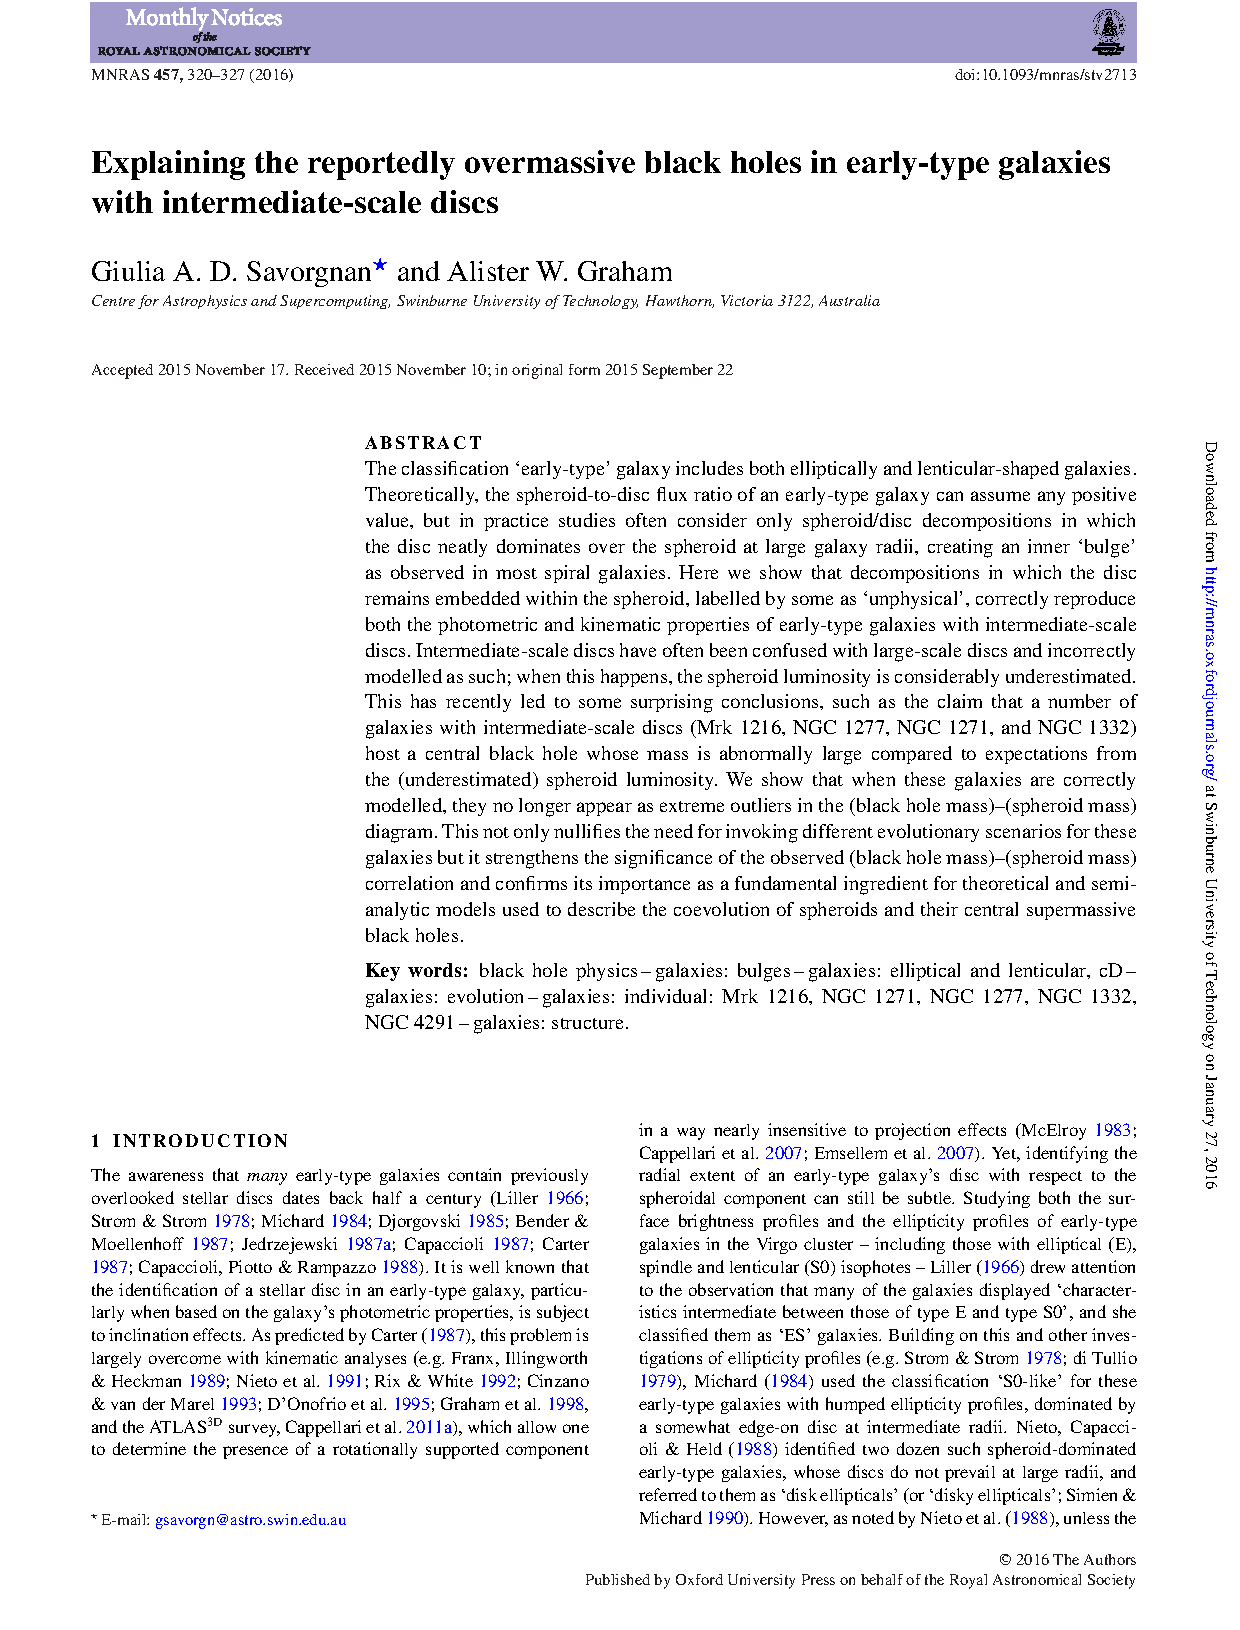
\includepdf[pages={1-8}]{MNRAS2016.pdf}
